
\zsavepos{header-1}

\zsavepos{header-1}\section{Dataset\zsavepos{header-2\zsavepos{header-2}}
\zsavepos{header-3}\zlabel{header}
}\zsavepos{header-3}\zlabel{header}

\label{sec:data}
It is too costly to conduct an expert annotation of optimal procedural graphs for a large number of documents. To this end, we build our dataset upon a model collection of business process~\cite{dumas2018fundamentals}, which has defined optimal procedural graphs covering the whole business process management lifecycle. The dataset construction turns into a data2text task --- generates suitable documents for given procedural graphs.

\zsavepos{header-1}

\zsavepos{header-1}\subsection{Preliminary\zsavepos{header-2\zsavepos{header-2}}
\zsavepos{header-3}\zlabel{header}
}\zsavepos{header-3}\zlabel{header}

Figure~\ref{fig:task_b} presents an example of the optimal procedural graph. It describes the procedure of how a restaurant serves customers and involves two actors~(customer and restaurant).
Each actor starts from the ``Start'' node, carries out actions following the logic in the graph, and ends at the ``End'' node. If the actions are performed sequentially, they are connected by the ``Sequence Flow''. Otherwise, there is an ``Inclusive Gateway'', ``Exclusive Gateway'' or ``Parallel Gateway'' indicating the following actions are non-sequential ones. Both the ``Inclusive Gateway''~(G-1) and ``Exclusive Gateway''~(G-3) mean that the following action is performed under the condition on the connected ``Condition Flow''. The difference is that there is one and only one condition after the ``Exclusive Gateway'' can be met, while this does not apply to the ``Inclusive Gateway''. The ``Parallel Gateway''~(G-5) represents that the following actions are performed in parallel. Note that, all gateways appear in pairs and the latter ones~(G-4, G-2, G-6) indicate the end of the non-sequential activities. Additionally, the ``Data Constraint'' and ``Action Constraint'' represent the necessary data~(C-1) and essential notices~(C-2) for actions connected by the ``Constraint Flow'', respectively.

\zsavepos{header-1}

\zsavepos{header-1}\subsection{Dataset Construction\zsavepos{header-2\zsavepos{header-2}}
\zsavepos{header-3}\zlabel{header}
}\zsavepos{header-3}\zlabel{header}

With these high-quality procedural graphs, we then perform the dataset construction as a data2text task~\cite{lin2023survey}. Specifically, {we design a three-stage pipeline: 1) Decomposition \& Transformation that decomposes the graph into fragmented spans/sentences in natural language; 2) Grouping \& Ordering that logically organizes the procedural fragments; 3) Aggregating \& Smoothing that unifies the fragments into high-quality documents}.

\zsavepos{header-1}\paragraph{Decomposition \& Transformation\zsavepos{header-2}}\zsavepos{header-3}\zlabel{header}

To narrow the huge gap between the complex graph and the length document, we first decompose the graph into minimal meaningful units. We define a vocabulary with nineteen units, each of which consists of actions, gateways or constraints connected by flow~(cf., Appx.~\ref{app:DT}). We also design nineteen hand-written templates for the vocabulary. Based on the unit vocabulary, we perform the breadth-first search strategy~\cite{10.1016/0004-3702(85)90084-0} over the graph, as shown in Figure~\ref{fig:Decomposition}. Particularly, some actions may be repeatedly walked to preserve the sequential execution relation between adjacent actions in the graph. For example, ``Order drinks'' is walked twice, forming ``If need drinks, then order drinks.'' and ``Order drinks, then specify the size.''. We then transform the decomposed units into natural language spans/sentences based on the paired templates. We call these spans/sentences ``procedural fragments''.

\begin{figure}[t]
    \zsavepos{figure-1}
    \zsavepos{figure-1}
    \centering
    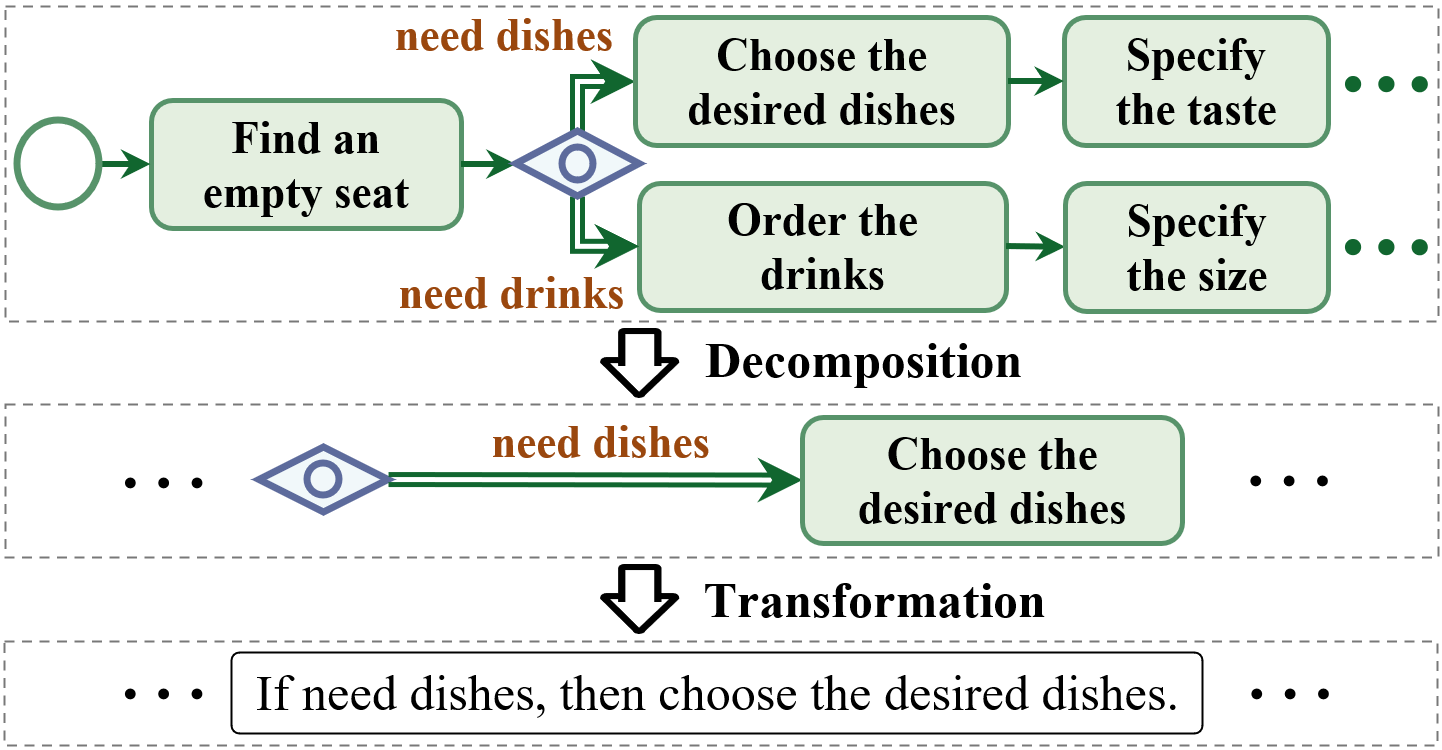
\includegraphics[width=1\linewidth]{figures/dataset/DatasetConstruction_1.png}
    \zsavepos{figure-2}

    \zsavepos{figure-2}
    \zsavepos{figurecap-1}
    \zsavepos{figurecap-1}\caption{Illustration of decomposing the graph into units and transforming a unit into a procedural fragment.
    }\zsavepos{figurecap-2}\zsavepos{figurecap-2}
    \label{fig:Decomposition}
    \zlabel{figure}

    \zlabel{figure}
\end{figure}
\vspace{5pt}

\begin{figure}[t]
    \zsavepos{figure-1}
    \zsavepos{figure-1}
    \centering
    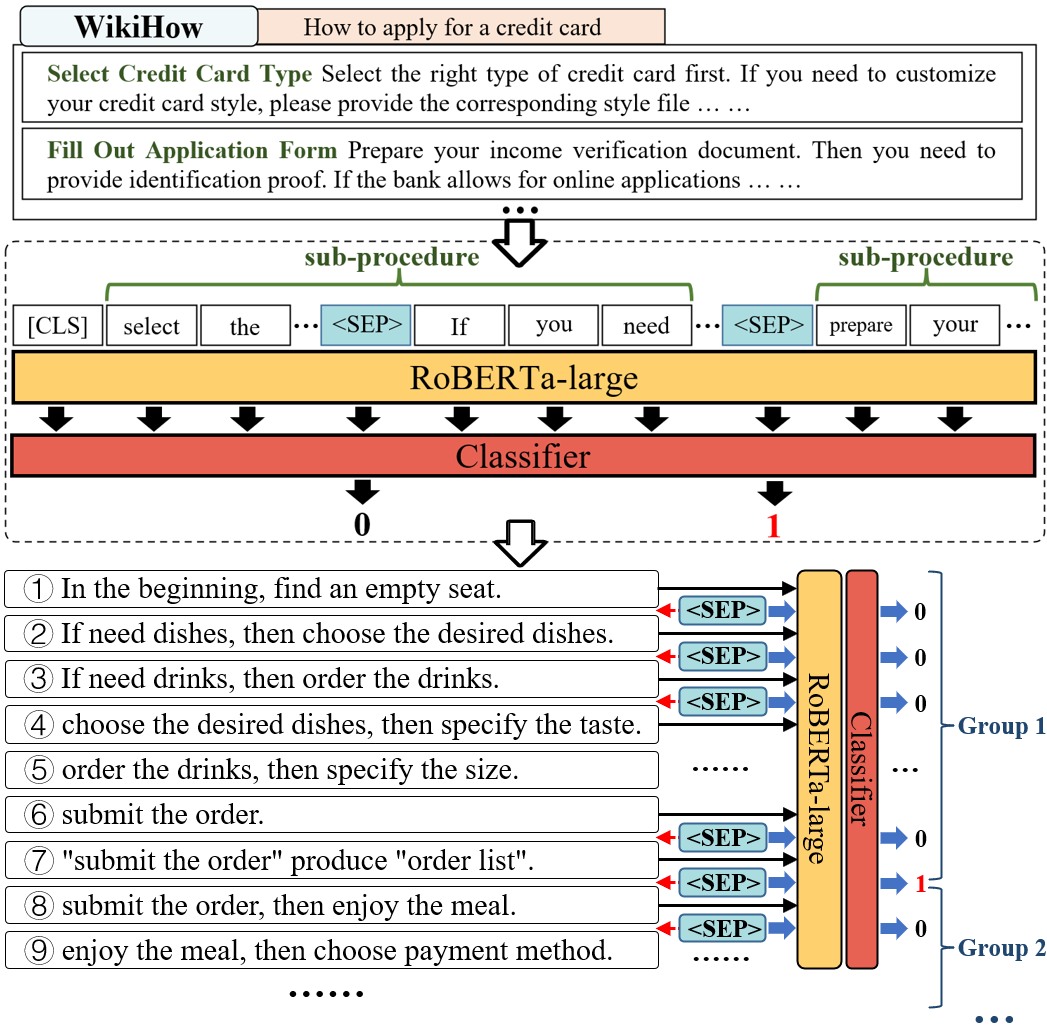
\includegraphics[width=1\linewidth]{figures/dataset/DatasetConstruction_2.png}
    \zsavepos{figure-2}

    \zsavepos{figure-2}
    \zsavepos{figurecap-1}
    \zsavepos{figurecap-1}\caption{The grouping of procedural fragments using a pre-trained boundary identification model.}\zsavepos{figurecap-2}\zsavepos{figurecap-2}
    \label{fig:Grouping_Ordering}
    \zlabel{figure}

    \zlabel{figure}
\end{figure}
\vspace{5pt}

\zsavepos{header-1}\paragraph{Grouping \& Ordering\zsavepos{header-2}}\zsavepos{header-3}\zlabel{header}

When writing a procedural document, it is vital to provide information in a logical way, namely, describing the whole procedure sub-procedure by sub-procedure~\cite{futrelle1999summarization, futrelle2004handling}. Hence, we need to group the fragments into sub-procedures. Specifically, we employ a simple boundary identification model, which employs the RoBERTa-large model~\cite{liu2019roberta} with a classifier layer, to predict whether a fragment is the end of a group. We train it on the WikiHow corpus~\citet{bolotova2023wikihowqa}, which consists of procedural documents collected from the \href{https://www.wikihow.com/}{WikiHow} website and format marks indicate different sub-procedures. The pre-trained model is then used to assign group marks for fragments, cf., Figure~\ref{fig:Grouping_Ordering}.
It is worth noticing that the way people describe a procedure is not the way the machine searches over the graph. Thus, it is necessary to order the fragments to better match human expression. For example, we need to exchange fragment \ding{194} and fragment\ding{195} of Group 1 in Figure~\ref{fig:Grouping_Ordering}. We achieve this via a fragment ordering model, whose structure is borrowed from~\citet{bin2023non}. Besides the WikiHow documents, we train this model on the remaining publicly
available procedural document datasets~\cite{castelli2020techqa, zhang-etal-2020-reasoning, lyu2021goal,sakaguchi2021proscript, nandy2021question} to reorder sentences after random shuffle. We use the pre-trained model to determine the order of fragments in the same group.

\zsavepos{header-1}\paragraph{Aggregating \& Smoothing\zsavepos{header-2}}\zsavepos{header-3}\zlabel{header}

In a standard procedural document, a single sentence~(``If the customer needs dishes, then choose the desired dishes and specify the taste.'') may convey multiple procedural fragments~(\ding{193} and \ding{195}). Given this, we reuse the boundary identification model to aggregate fragments that should be presented in the same sentence. The model is retrained to identify the correct ends of sentences from randomly inserted ones on the datasets used in the ordering phase. The pre-trained model is used to assign sentence marks for the fragments.
We further add the actor information before all fragments corresponding to each actor. At this point, all fragments have been organized in proper order with group and sentence marks. We paraphrase the fragments via ChatGPT, which has shown near or even superior human-level performance in many paraphrasing task~\cite{chui2023chatgpt}. After paraphrasing, we notice that there are a small number of redundant expressions caused by repeatedly walked nodes and inconsistent actions/constraints generated by ChatGPT. Thus, we further refine the documents with a few handwriting rules and manual corrections. At last, we develop a dataset with 3,394 high-quality document-graph pairs. On average, each document contains 10.67 sentences and each sentence contains 15.22 words. See Table~\ref{dataset:statistics} in Appx.~\ref{app:Aggregating_Smoothing} for more statistics.

\zsavepos{header-1}

\zsavepos{header-1}\subsection{Dataset Analysis\zsavepos{header-2\zsavepos{header-2}}
\zsavepos{header-3}\zlabel{header}
}\zsavepos{header-3}\zlabel{header}

\label{Dataset Quality Evaluation}
We analyze our datasets to investigate whether the generated procedural documents are consistent with the original graphs, whether the documents are qualified according to human standards, and whether the proposed strategies contribute to a better quality of the dataset. Therefore, we conduct both automatic and human evaluations to compare the dataset constructed by our three-stage pipeline with the datasets constructed by two variations.

\zsavepos{header-1}\paragraph{Automatic Evaluation\zsavepos{header-2}}
\zsavepos{header-3}\zlabel{header}
 We adopt two commonly used Data2Text metrics. The \textit{FINE} score~\cite{faille2021entity} models the evaluation as a natural language inference task --- by inferring fragments from the documents it checks omissions, while the other direction checks hallucinations. The \textit{ESA} score~\cite{faille2021entity} evaluates the coverage of entities and actions in the documents. For both, higher values indicate better performance. Details are listed in the appendix~\ref{app:AutomaticEvaluation}.

\zsavepos{header-1}\paragraph{Human Evaluation\zsavepos{header-2}}
\zsavepos{header-3}\zlabel{header}
 Inspired by~\citet{miller1979humanistic}, we ask three workers to score the document from 1 to 5 on five criteria:
\textit{readability}, the quality of the document to be understood easily;
\textit{accuracy}, the quality of the document accurately describing the information in the procedure graph;
\textit{clarity}, the quality of the document expressing the complex execution of actions logically;
\textit{simplicity}, the quality of the document not containing redundant information;
\textit{usability}, the quality of the document aiding users in accomplishing this procedure.
Details are listed in the appendix~\ref{app:HumanEvaluation}.

\zsavepos{header-1}\paragraph{Variations\zsavepos{header-2}}
\zsavepos{header-3}\zlabel{header}
 We create two variants of our three-stage pipeline: \textit{concatenating}, which directly concatenates all fragments to form the documents; \textit{paraphrasing}, which directly paraphrases the concatenation of all fragments using ChatGPT without grouping, ordering and aggregating process.
Note that, we don't involve \textit{concatenating} in the automatic evaluation. This is because the concatenation of all fragments is always consistent with the information in the graphs but lacks fluency and logicality which requires further human evaluation.
\begin{figure}[t]
    \zsavepos{figure-1}
    \zsavepos{figure-1}
    \centering
    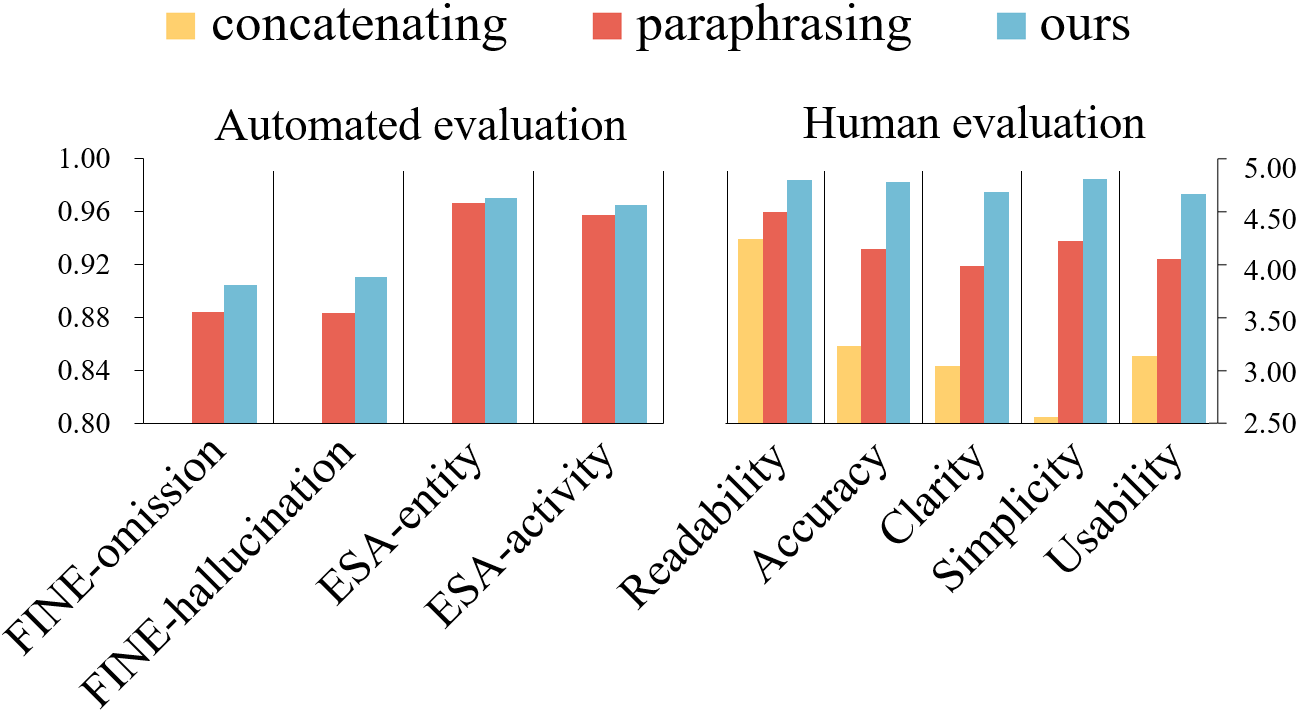
\includegraphics[width=1\linewidth]{figures/dataset/DatasetEva_Human.png}
    \zsavepos{figure-2}

    \zsavepos{figure-2}
    \zsavepos{figurecap-1}
    \zsavepos{figurecap-1}\caption{Comparison of our method with two variations via automatic and human evaluations.}\zsavepos{figurecap-2}\zsavepos{figurecap-2}
    \label{fig:DatasetEva&Human}
    \zlabel{figure}

    \zlabel{figure}
\end{figure}

% Please add the following required packages to your document preamble:
% \usepackage{multirow}

\begin{table*}[t]
\caption{Performances of state-of-the-art baselines and LLMs. Higher values indicate better performances.}
\label{exp_results}
\centering
\scalebox{0.65}{
\begin{tabular}{clcccccccccc}
\hline
\multicolumn{1}{c|}{\multirow{2}{*}{\textbf{Row}}} & \multicolumn{1}{c|}{\multirow{2}{*}{\textbf{Model}}} & \multicolumn{1}{c|}{\multirow{2}{*}{\textbf{Actor}}} & \multicolumn{1}{c|}{\multirow{2}{*}{\textbf{Action}}} & \multicolumn{2}{c|}{\textbf{Constraint}}              & \multicolumn{3}{c|}{\textbf{Gateway}}                                            & \multicolumn{3}{c}{\textbf{Flow}}                            \\ \cline{5-12} 
\multicolumn{1}{c|}{}                              & \multicolumn{1}{c|}{}                                & \multicolumn{1}{c|}{}                                & \multicolumn{1}{c|}{}                                 & \textbf{Data}  & \multicolumn{1}{c|}{\textbf{Action}} & \textbf{Exclusive} & \textbf{Inclusive} & \multicolumn{1}{c|}{\textbf{Parallel}} & \textbf{Sequence} & \textbf{Condition} & \textbf{Constraint} \\ \hline
\multicolumn{1}{c|}{1}                             & \multicolumn{1}{l|}{\citet{sonbol2023machine}}               & \multicolumn{1}{c|}{0.028}                           & \multicolumn{1}{c|}{0.308}                            & 0.213          & \multicolumn{1}{c|}{-}               & 0.485              & -                  & \multicolumn{1}{c|}{0.279}             & 0.056             & 0.047              & 0.017               \\ \cline{2-12} 
\multicolumn{1}{c|}{2}                             & \multicolumn{1}{l|}{\citet{neuberger2023beyond}}             & \multicolumn{1}{c|}{0.027}                           & \multicolumn{1}{c|}{0.276}                            & -              & \multicolumn{1}{c|}{-}               & 0.469              & -                  & \multicolumn{1}{c|}{0.337}             & 0.074             & 0.061              & -                   \\ \cline{2-12} 
\multicolumn{1}{c|}{3}                             & \multicolumn{1}{l|}{\citet{sholiq2022generating}}            & \multicolumn{1}{c|}{-}                               & \multicolumn{1}{c|}{0.387}                            & -              & \multicolumn{1}{c|}{-}               & 0.463              & -                  & \multicolumn{1}{c|}{0.198}             & 0.091             & 0.022              & -                   \\ \cline{2-12} 
\multicolumn{1}{c|}{4}                             & \multicolumn{1}{l|}{PET~\cite{bellan2023pet}}                             & \multicolumn{1}{c|}{0.085}                           & \multicolumn{1}{c|}{0.430}                            & 0.069          & \multicolumn{1}{c|}{-}               & \underline{0.493}              & -                  & \multicolumn{1}{c|}{-}                 & 0.164             & 0.026              & 0.000                    \\ \cline{2-12} 
\multicolumn{1}{c|}{5}                            & \multicolumn{1}{l|}{CIS~\cite{bellan2022leveraging}}                             & \multicolumn{1}{c|}{0.633}                           & \multicolumn{1}{c|}{0.639}                            & -              & \multicolumn{1}{c|}{-}               & 0.455              & -                  & \multicolumn{1}{c|}{-}                 & 0.203             & 0.157              & -                   \\ \hline
\multicolumn{1}{l|}{}                              & \multicolumn{1}{l|}{Flan-T5~\cite{chung2022scaling}}                         & \multicolumn{1}{c|}{}                                & \multicolumn{1}{c|}{}                                 &                & \multicolumn{1}{c|}{}                &                    &                    & \multicolumn{1}{c|}{}                  &                   &                    &                     \\
\multicolumn{1}{c|}{6}                             & \multicolumn{1}{l|}{\quad + Few-shot In-context Learning}               & \multicolumn{1}{c|}{0.206}                           & \multicolumn{1}{c|}{0.362}                            & -              & \multicolumn{1}{c|}{-}               & 0.376              & -                  & \multicolumn{1}{c|}{-}                 & 0.084             & 0.013              & -                   \\
\multicolumn{1}{c|}{7}                             & \multicolumn{1}{l|}{\quad + Supervised Fine-tuning}                     & \multicolumn{1}{c|}{\underline{0.659}}                           & \multicolumn{1}{c|}{\underline{0.684}}                            & 0.589          & \multicolumn{1}{c|}{\underline{0.366}}           & 0.419              & 0.045              & \multicolumn{1}{c|}{\underline{0.393}}             & 0.395             & \underline{0.168}              & 0.363               \\ \hline
\multicolumn{1}{l|}{}                             & \multicolumn{1}{l|}{ChatGPT~\cite{ouyang2022training}}                         &  \multicolumn{1}{c|}{}                                 & \multicolumn{1}{c|}{}                                 &                & \multicolumn{1}{c|}{}                &                    &                    & \multicolumn{1}{c|}{}                  &                   &                    &                     \\

\multicolumn{1}{c|}{8}                             & \multicolumn{1}{l|}{\quad + Few-shot In-context Learning} &\multicolumn{1}{c|}{0.625}                           & \multicolumn{1}{c|}{0.681}                            & \underline{0.687}          & \multicolumn{1}{c|}{0.286}           & 0.477              & \textbf{0.173}     & \multicolumn{1}{c|}{0.388}             & \underline{0.408}             & 0.158              & 0.\underline{444}               \\ \hline
\multicolumn{1}{l|}{}                              & \multicolumn{1}{l|}{Llama2~\cite{touvron2023llama}}                          & \multicolumn{1}{c|}{}                                & \multicolumn{1}{c|}{}                                 &                & \multicolumn{1}{c|}{}                &                    &                    & \multicolumn{1}{c|}{}                  &                   &                    &                     \\
\multicolumn{1}{c|}{9}                             & \multicolumn{1}{l|}{\quad + Few-shot In-context Learning}               & \multicolumn{1}{c|}{0.502}                           & \multicolumn{1}{c|}{0.573}                            & 0.357          & \multicolumn{1}{c|}{0.049}           & 0.446              & 0.067              & \multicolumn{1}{c|}{0.128}             & 0.193             & 0.107              & 0.201               \\
\multicolumn{1}{c|}{10}                            & \multicolumn{1}{l|}{\quad + Supervised Fine-tuning}                     & \multicolumn{1}{c|}{\textbf{0.674}}                  & \multicolumn{1}{c|}{\textbf{0.744}}                   & \textbf{0.779} & \multicolumn{1}{c|}{\textbf{0.499}}  & \textbf{0.554}     & \underline{0.090}              & \multicolumn{1}{c|}{\textbf{0.398}}    & \textbf{0.478}    & \textbf{0.319}     & \textbf{0.467}      \\ \hline
\multicolumn{12}{l}{\small * The best results are marked in bold, and the second-best results are marked with underlines.}                                                                                                                                                                                                                                                                                                                 
\end{tabular}
}
\vspace{5pt}
\end{table*}

% ~\citet{sonbol2023machine}
% ~\citet{neuberger2023beyond}
% ~\citet{bellan2022leveraging}
% PET~\citet{bellan2023pet}
% CIS~\citet{bellan2022leveraging}


% \begin{table*}[t]
% \caption{Performances of state-of-the-art baselines and LLMs. Higher values indicate better performances.}
% \label{exp_results}
% \centering
% \scalebox{0.68}{
% \begin{tabular}{l|c|c|cc|ccc|cccll}
% \cline{1-11}
% \multicolumn{1}{c|}{\multirow{2}{*}{\textbf{Model}}}                                                             & \multirow{2}{*}{\textbf{Actor}}             & \multirow{2}{*}{\textbf{Action}}            & \multicolumn{2}{c|}{\textbf{Constraint}}                                                                                           & \multicolumn{3}{c|}{\textbf{Gateway}}                                                                                   & \multicolumn{3}{c}{\textbf{Flow}}                                                                                                                                                                           & \multicolumn{1}{c}{} & \multicolumn{1}{c}{} \\ \cline{4-11}
% \multicolumn{1}{c|}{}                                                                                   &                                    &                                    & \textbf{\makecell{Data}} & \textbf{\makecell{Action}} & \textbf{Exclusive} & \textbf{Inclusive} & \textbf{Parallel} & \textbf{\makecell{Sequence}} & \textbf{\makecell{Condition}} & \textbf{\makecell{Constraint}} &                      &                      \\  \cline{1-11}
% [1] \citet{sonbol2023machine}                                                                         & 0.028                              & 0.308                              & 0.213                                                      & -                                                          & 0.485                               & -                                 & 0.279                              & 0.056                                                          & 0.047                                                           & 0.017                                                            &                      &                      \\
% \cline{1-11}
% [2] \citet{neuberger2023beyond}                                                                              & 0.027                              & 0.276                              & -                                                        & -                                                          & 0.469                               & -                                 & 0.337                              & 0.074                                                          & 0.061                                                           & -                                                              &                      &                      \\ 
% \cline{1-11}
% [3] \citet{sholiq2022generating}                                                                               & -                                & 0.387                              & -                                                        & -                                                          & 0.463                               & -                                 & 0.198                              & 0.091                                                          & 0.022                                                           & -                                                              &                      &                      \\
% \cline{1-11}
% [4] CIS~\cite{bellan2022leveraging}                                                                                      & 0.633                              & 0.639                              & -                                                        & -                                                          & 0.455                               & -                                 & -                                & 0.203                                                          & 0.157                                                           & -                                                              &                      &                      \\
% \cline{1-11}
% [5] PET~\cite{bellan2023pet}                                                                                      & 0.085                              & 0.430                              & 0.069                                                      & -                                                          & \underline{0.493}  & -                                 & -                                & 0.164                                                          & 0.026                                                           & -                                                              &                      &                      \\ 
% \cline{1-11}
% \cline{1-11}

% Flan-T5~\cite{chung2022scaling} &&&&&&&&&&& & \\
 
% [6] \quad + Few-shot Learning& 0.206 & 0.362 & - & - & 0.376 & - & - & 0.084 & 0.013 & - &                    &                      \\ 

% [7] \quad + Fine-tuning& \underline{0.659} & \underline{0.684} & 0.589                                                      & \underline{0.366}                           & 0.419                               & 0.045                               & \underline{0.393} & 0.395                                                          & \underline{0.168}                              & 0.363                                                            &                      &                      \\ 
%  \cline{1-11}
% [8] ChatGPT~\cite{ouyang2022training}                                                                                 & 0.625                              & 0.681                              & \underline{0.687}                         & 0.286                                                        & 0.477                               & \textbf{0.173}     & 0.388                              & \underline{0.408}                             & 0.158                                                           & \underline{0.444}                               &                      &                      \\
%  \cline{1-11}
%  Llama2~\cite{touvron2023llama}&&&&&&&&&&& & \\

% [9] \quad + Few-shot Learning& 0.502                              & 0.573                              & 0.357                                                      & 0.049                                                        & 0.446                               & 0.067                               & 0.128                              & 0.193                                                          & 0.107                                                           & 0.201                                                            &                      &                      \\

% [10] \quad + Fine-tuning                                                                     & \textbf{0.674}    & \textbf{0.744}    & \textbf{0.779}                            & \textbf{0.499}                              & \textbf{0.554}     & \underline{0.090}  & \textbf{0.398}    & \textbf{0.478}                                & \textbf{0.319}                                 & \textbf{0.467}                                  &                      &                      \\ 
% \cline{1-11}
% \multicolumn{11}{l}{\small * The best results are marked in bold, and the second-best results are marked with underlines.} &&\\
% \end{tabular}}
% \end{table*}

% \begin{table*}[!th]
% \caption{Experimental results of the baseline models. The best results are represented in bold, and the second best results are highlighted with an underline. For simplicity, we use ``XOR'', ``OR'' and ``AND'' as abbreviations for exclusive, inclusive and parallel gateways respectively.}
% \label{exp_results}
% \centering
% \scalebox{0.72}{
% \begin{tabular}{l|c|ccc|cc|ccc|c}
% \hline
% \multicolumn{1}{c|}{\multirow{3}{*}{\textbf{Model}}} & \multirow{3}{*}{\textbf{Action}} & \multicolumn{3}{c|}{\textbf{Gateway}}               & \multicolumn{2}{c|}{\textbf{Constraint}}            & \multicolumn{3}{c|}{\textbf{Flow}}                                       & \multirow{3}{*}{\textbf{Actor}} \\ \cline{3-10}
% \multicolumn{1}{c|}{}                                &                                  & \textbf{XOR}    & \textbf{OR}     & \textbf{AND}    & \textbf{\makecell{Data\\Constraint}} & \textbf{\makecell{Action\\Constraint}} & \textbf{\makecell{Sequence\\Flow}} & \textbf{\makecell{Condition\\Flow}} & \textbf{\makecell{Constraint\\Flow}} &                                 \\ \hline
% \uppercase\expandafter{\romannumeral1}. Pipeline Based                                       &                                  &                 &                 &                 &                         &                           & \textbf{}             & \textbf{}              &                         &                                 \\
% \ Translation Like                                     & 0.308                           & 0.485          &---              & 0.279          & 0.213                  &---                         & 0.056                & 0.047                 & 0.017                  & 0.028                          \\
% \ Beyond Rule                                          & 0.276                           & 0.469          &---              & 0.337          &---                      &---                        & 0.074                & 0.061                 &---                      & 0.027                          \\ \hline
% \uppercase\expandafter{\romannumeral2}. Elements Linking                                     &                                  &                 &                 &                 &                         &                           &                       &                        &                         &                                 \\
% \ Fact Types                                           & 0.387                           & 0.463          &---              & 0.198          &---                      &---                        & 0.091                & 0.022                &---                      &---                              \\
% \ PET                                                  & 0.430                           & \underline{0.493}          &---              &---              & 0.069                  &---                        & 0.164                & 0.026                 &---                      & 0.085                          \\
% \ CIS                                                  & 0.639                           & 0.455          &---              &---              &---                      &---                        & 0.203                & 0.157                 &---                      & 0.633                          \\ \hline
% \uppercase\expandafter{\romannumeral3}. End to End                                           &                                  &                 &                 &                 &                         &                           &                       &                        &                         &                                 \\
% \ Flan-T5 fine-tuned                                   & \underline{0.684}                           & 0.419          & 0.045          & \underline{0.393}          & 0.589                  & \underline{0.366}                    & 0.395                & \underline{0.168}                 & 0.363                  & \underline{0.659}                          \\
% \ ChatGPT                                              & 0.681                           & 0.477          & \textbf{0.173} & 0.388          & \underline{0.687}                  & 0.286                    & \underline{0.408}                & 0.158                 & \underline{0.444}                  & 0.625                          \\
% \ Llama2 few-shot                                      & 0.573                           & 0.446          & 0.067          & 0.128          & 0.357                  & 0.049                    & 0.193                & 0.107                 & 0.201                  & 0.502                          \\
% \ Llama2 fine-tuned                                    & \textbf{0.744}                  & \textbf{0.554} & \underline{0.090}          & \textbf{0.398} & \textbf{0.779}         & \textbf{0.499}           & \textbf{0.478}       & \textbf{0.319}        & \textbf{0.467}         & \textbf{0.674} \\ \hline          
% \end{tabular}
% }
% \end{table*}
% \begin{table*}[!th]
% \caption{Experimental results of the baseline models. The best results are represented in bold, and the second best results are highlighted with an underline. For simplicity, we use ``XOR'', ``OR'' and ``AND'' as abbreviations for exclusive, inclusive and parallel gateways respectively.}
% \label{exp_results}
% \centering
% \scalebox{0.72}{
% \begin{tabular}{l|c|ccc|cc|ccc|c}
% \hline
% \multicolumn{1}{c|}{\multirow{3}{*}{\textbf{Model}}} & \multirow{3}{*}{\textbf{Action}} & \multicolumn{3}{c|}{\textbf{Gateway}}               & \multicolumn{2}{c|}{\textbf{Constraint}}            & \multicolumn{3}{c|}{\textbf{Flow}}                                       & \multirow{3}{*}{\textbf{Actor}} \\ \cline{3-10}
% \multicolumn{1}{c|}{}                                &                                  & \textbf{XOR}    & \textbf{OR}     & \textbf{AND}    & \textbf{\makecell{Data\\Constraint}} & \textbf{\makecell{Action\\Constraint}} & \textbf{\makecell{Sequence\\Flow}} & \textbf{\makecell{Condition\\Flow}} & \textbf{\makecell{Constraint\\Flow}} &                                 \\ \hline
% \uppercase\expandafter{\romannumeral1}. Pipeline Based                                       &                                  &                 &                 &                 &                         &                           & \textbf{}             & \textbf{}              &                         &                                 \\
% Translation Like                                     & 0.3079                           & 0.4848          &---              & 0.2786          & 0.2133                  &---                        & 0.0558                & 0.0468                 & 0.0172                  & 0.0276                          \\
% Beyond Rule                                          & 0.2757                           & 0.4685          &---              & 0.3369          &---                      &---                        & 0.0744                & 0.0611                 &---                      & 0.0266                          \\ \hline
% \uppercase\expandafter{\romannumeral2}. Elements Linking                                     &                                  &                 &                 &                 &                         &                           &                       &                        &                         &                                 \\
% Fact Types                                           & 0.3874                           & 0.4633          &---              & 0.1983          &---                      &---                        & 0.0910                & 0.0223                 &---                      &---                              \\
% PET                                                  & 0.4297                           & \underline{0.4932}          &---              &---              & 0.0689                  &---                        & 0.1640                & 0.0257                 &---                      & 0.0846                          \\
% CIS                                                  & 0.6393                           & 0.4549          &---              &---              &---                      &---                         & 0.2034                & 0.1574                 &---                      & 0.6326                          \\ \hline
% \uppercase\expandafter{\romannumeral3}. End to End                                           &                                  &                 &                 &                 &                         &                           &                       &                        &                         &                                 \\
% Flan-T5 fine-tuned                                   & \underline{0.6843}                           & 0.4188          & 0.0449          & \underline{0.3932}          & 0.5887                  & \underline{0.3661}                    & 0.3952                & \underline{0.1678}                 & 0.3626                  & \underline{0.6589}                          \\
% ChatGPT                                              & 0.6812                           & 0.4768          & \textbf{0.1729} & 0.3878          & \underline{0.6873}                  & 0.2859                    & \underline{0.4078}                & 0.1581                 & \underline{0.4442}                  & 0.6245                          \\
% Llama2 few-shot                                      & 0.5725                           & 0.4459          & 0.0672          & 0.1284          & 0.3571                  & 0.0492                    & 0.1927                & 0.1074                 & 0.2005                  & 0.5020                          \\
% Llama2 fine-tuned                                    & \textbf{0.7439}                  & \textbf{0.5539} & \underline{0.0900}          & \textbf{0.3979} & \textbf{0.7788}         & \textbf{0.4991}           & \textbf{0.4777}       & \textbf{0.3190}        & \textbf{0.4669}         & \textbf{0.6742}                
% \end{tabular}
% }
% \end{table*}

% \uppercase\expandafter{\romannumeral1}



\zsavepos{header-1}\paragraph{Results\zsavepos{header-2}}\zsavepos{header-3}\zlabel{header}

As shown in Figure~\ref{fig:DatasetEva&Human}, the proposed three-stage pipeline achieves better performance than the other two variations under both automatic and human evaluation. Automatic evaluation reveals that although the paraphrasing variation obtains almost close ESA scores to our pipeline, it loses the game completely on the FINE metrics without the help of grouping, ordering and aggregating strategies. From human evaluation, we further demonstrate the superiority of our pipeline to describe procedural graphs in a fluent, accurate, logical, simple, and user-friendly way. Specifically, the concatenating variation gets the lowest scores on all criteria due to its inaction of unreadable spans, redundant information, and chaotic orders. In line with the automatic evaluation, we observe the largest gap between the paraphrasing variation and our pipeline on the clarity criterion due to its invisibility of complex logic among the fragments. Note that, the ICC scores of all evaluations are above 0.75, indicating the reliability of human results~\cite{koo2016guideline}.
